\subsection{Webstránka}
\label{webstranka}
Webstránka sama o sebe nemá zmysel. Slúži výhradne na prístup k dátam poslaným pomocou Outsidera v applikácii Passer.

Úvodná obrazovka ponúka používateľovi verifikovať sa buď pomocou šesťciferného kódu, alebo pomocou QR kódu. 

Počas zadávania šesťciferného kódu sa jednotlivé číslice ukladajú do poľa. Keď je naplnené (dĺžka poľa musí byť 6), prebehne serializácia do JSON štruktúry a kód sa posiela na server. Ten ho skontroluje a vráti odpoveď webstránke. Opäť: bližší rozbor (vrátane skenovania QR kódu) v \nameref{vzajomne_interakcie}.

Po úspešnej verifikácii je používateľ presmerovaný do sekcie, kde sa mu zobrazia všetky položky z Passera, ktoré si cez Outsider poslal. Z tejto obrazovky je možné skopírovať jednotlivé atribúty položiek (tlačidlo \textit{COPY}). Pri položkách typu heslo je možnosť aj priamo prejsť na webstránku uvedenú v položke pomocou tlačidla \textit{VISIT WEB}. 

\begin{figure}[H]
  \centering
  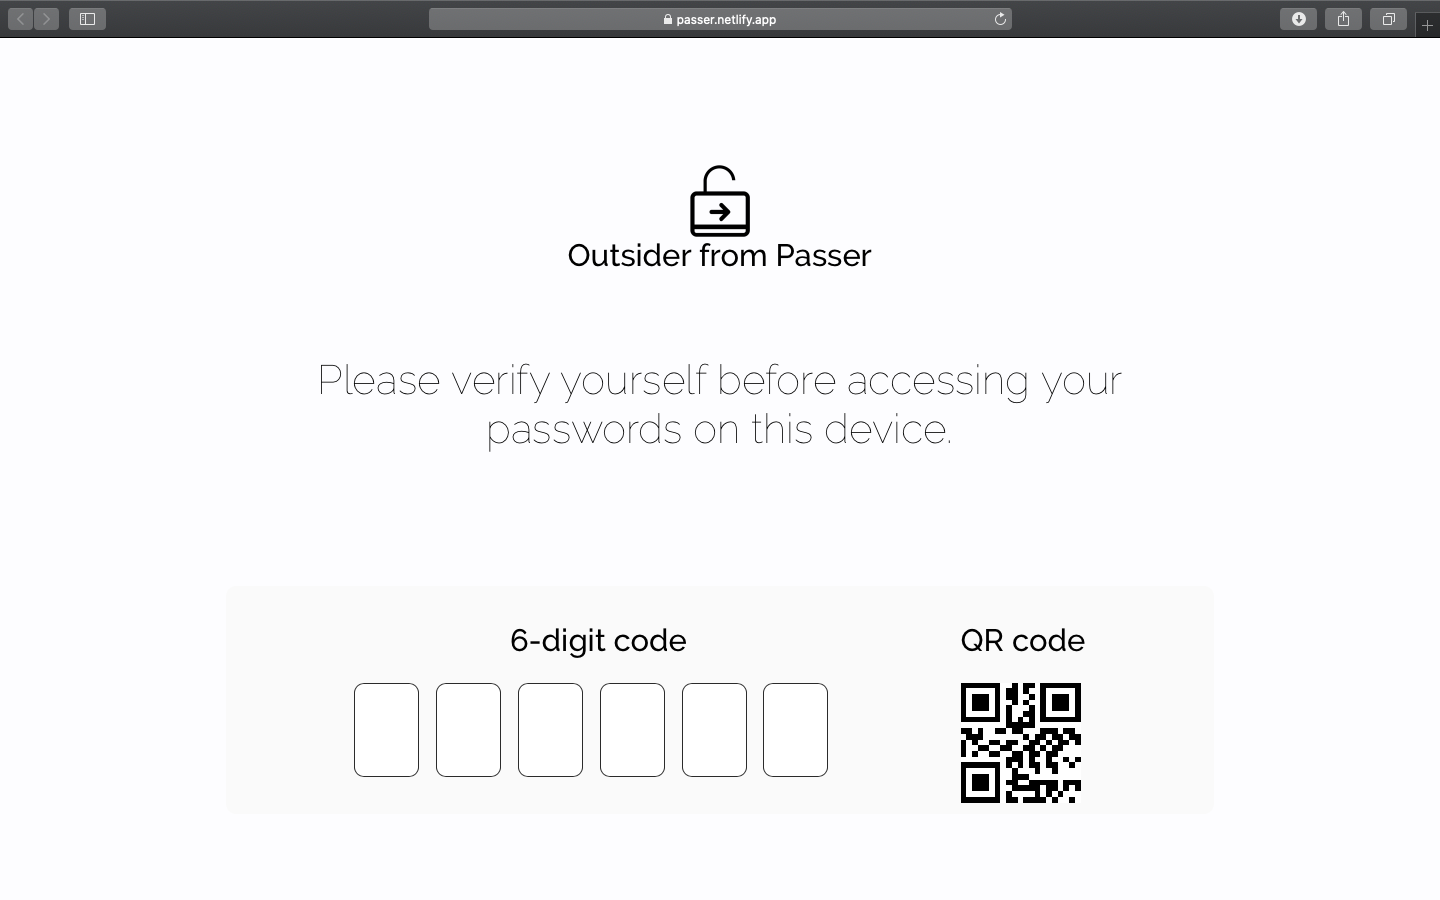
\includegraphics[width=15cm]{img/website1.png}
  \caption{Webstránka - Úvodná obrazovka.}
  \label{website1}
\end{figure}

\begin{figure}[H]
  \centering
  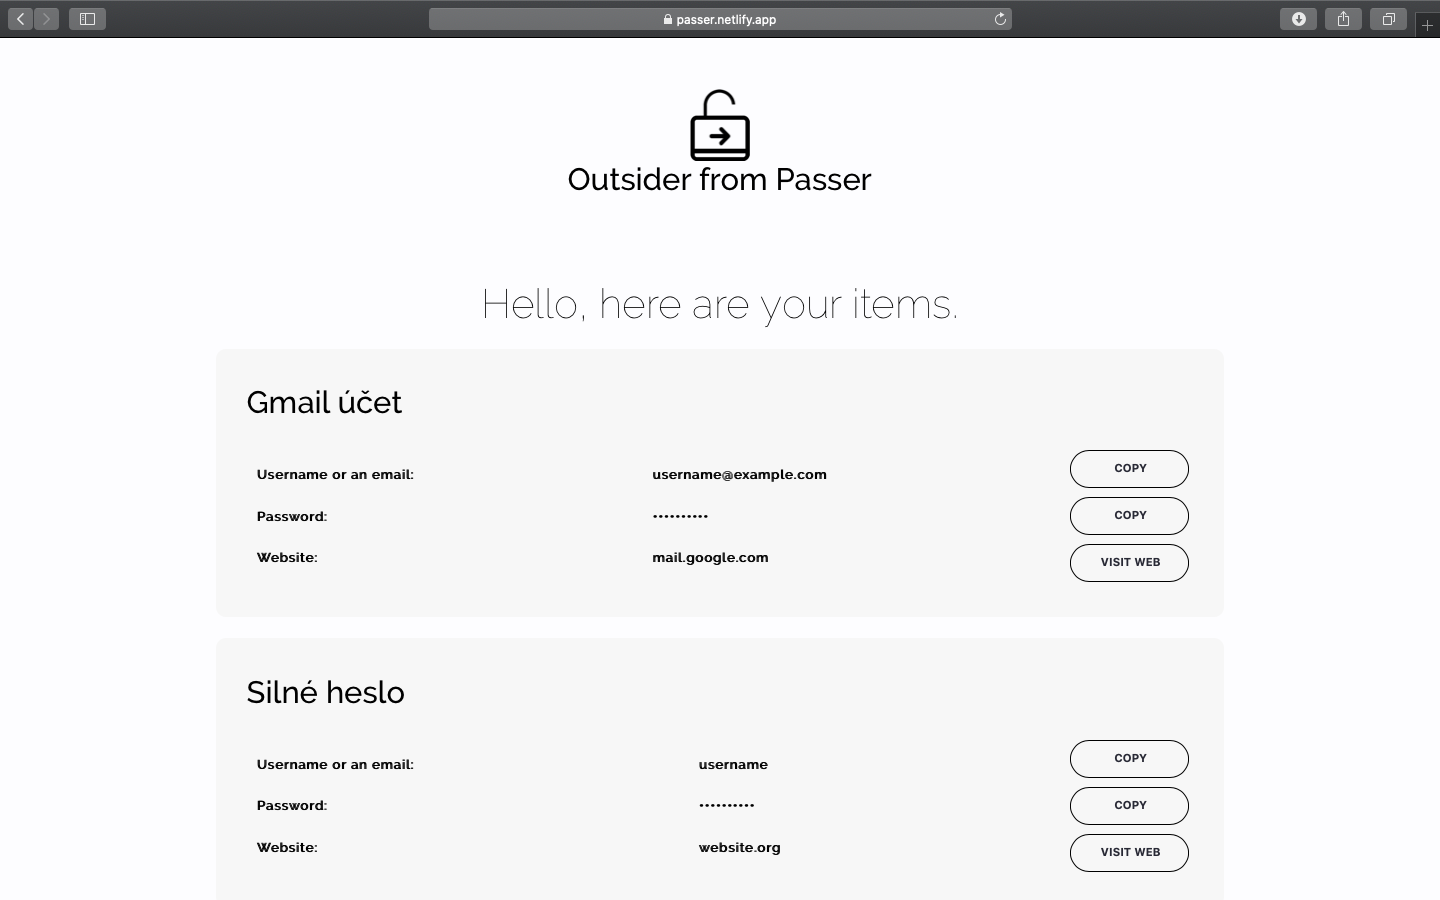
\includegraphics[width=15cm]{img/website2.png}
  \caption{Webstránka - Zobrazenie Passer položiek.}
  \label{website2}
\end{figure}